\documentclass[crop,tikz]{standalone}
\usetikzlibrary{mindmap}
%\setlength\parindent{0pt}
\renewcommand{\footnotesize}{\fontsize{5.5}{6.0}\selectfont}
\renewcommand{\normalsize}{\fontsize{7.5}{11.0}\selectfont}
\begin{document}
	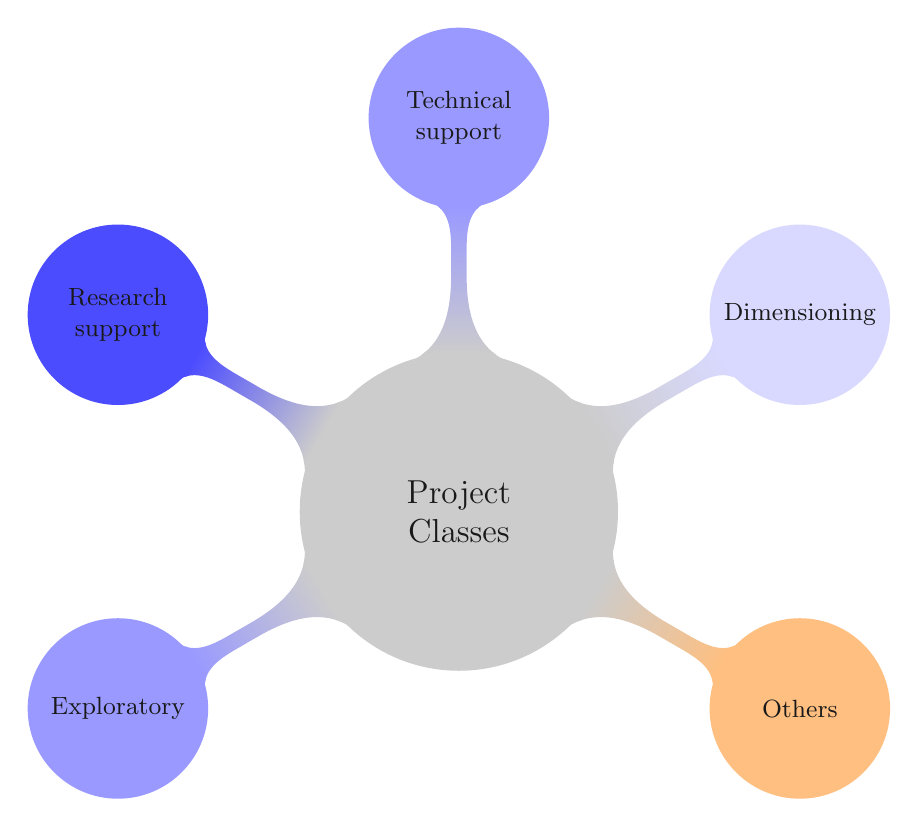
\begin{tikzpicture}
		\path[
		mindmap,
		concept color=gray!40,
		text=black!90
		] {
			node[concept] {Project\\Classes} [clockwise from=210]
			child[concept color=blue!40]  { 
				node[concept] {Exploratory}
			}
			child[concept color=blue!70]  { 
				node[concept] {Research support} 
			}
			child[concept color=blue!40]   {
				node[concept] {Technical support}
			}
			child[concept color=blue!15]   {
				node[concept] {Dimensioning}
			}
			child[concept color=orange!50]   {
				node[concept] {Others}
			}
		};
	\end{tikzpicture}
\end{document}